This section explains how \app{} turns the drawing and zone settings into momentary
currents, then works through the two-zone demonstration by hand.
Section~\ref{sec:testing} describes how the calculation was checked.

\subsection{Terms}

\begin{description}[style=nextline, leftmargin=1.2em]
  \item[Zone (event)] One protection scheme operating for a fault in its zone. Each
    zone is a separate event: faults in different zones are never added together,
    even where the zones overlap and share a breaker.
  \item[Stage] A step within an event: primary trip, backup trip, breaker failure,
    reclose, motor inrush or motor run. Loads in the same stage of a zone operate
    \emph{simultaneously} and are added together. Different stages happen at different
    times and are reported separately.
  \item[Load] One coil or motor current of one device, assigned to a stage.
  \item[DC supply] The battery or DC bus that feeds a coil, for example \emph{DC 1}.
    Each supply's current is calculated and reported separately; supplies are never
    combined into a single total.
\end{description}

Figure~\ref{fig:calcflow} summarizes the calculation.

\begin{figure}[H]
  \centering
  \begin{tikzpicture}[
      node distance=5mm and 8mm,
      box/.style={rectangle, rounded corners=3pt, draw=gftgreen, fill=gftlight, align=center,
                  font=\small, text width=37mm, minimum height=14mm},
      arr/.style={-{Stealth[length=2.5mm]}, line width=0.8pt, color=gftgreen!80!black}]
    \node[box] (a) {\textbf{Load rows}\\device, coil, stage, operation};
    \node[box, right=of a] (b) {\textbf{Row current}\\$I_{\text{row}} = n \times I_{\text{unit}}$\\(Eq.~\ref{eq:row})};
    \node[box, right=of b] (c) {\textbf{Stage total per supply}\\sum of simultaneous rows\\(Eq.~\ref{eq:stage})};
    \node[box, below=of c] (d) {\textbf{Supply peak}\\largest stage total over complete zones (Eq.~\ref{eq:peak})};
    \node[box, left=of d] (e) {\textbf{Completeness}\\verified, nothing to review};
    \node[box, left=of e] (f) {\textbf{Report}\\COMPLETE, or provisional};
    \draw[arr] (a) -- (b);
    \draw[arr] (b) -- (c);
    \draw[arr] (c) -- (d);
    \draw[arr] (e) -- (d);
    \draw[arr] (d.south) -- ++(0,-4mm) -| (f.south);
  \end{tikzpicture}
  \caption{From load rows to the supply peaks}
  \label{fig:calcflow}
\end{figure}

\subsection{Row Currents and Multipliers}\label{sec:calcmultipliers}

Each load row's current is the device's entered current, $I_{\text{unit}}$,
multiplied by the number of coils that operate, $n$:

\begin{equation}
  I_{\text{row}} = n \times I_{\text{unit}}, \qquad
  n = \begin{cases}
        N_{\text{poles}} & \text{all-pole operation of a breaker coil with}\\
                          & \text{per-mechanism current and independent mechanisms}\\
        1 & \text{otherwise}
      \end{cases}
  \label{eq:row}
\end{equation}

\begin{table}[H]
  \centering
  \caption{Multiplier $n$ for breaker coils}
  \label{tab:multiplier}
  \begin{tabularx}{\textwidth}{l l l c L}
    \toprule
    \textbf{Current basis} & \textbf{Mechanisms} & \textbf{Operation} & $n$ & \textbf{Example, 3 poles at 10 A} \\
    \midrule
    Whole breaker & Shared & All poles & 1 & 10 A \\
    Per mechanism & Shared & All poles & 1 & 10 A \\
    Per mechanism & Independent & All poles & 3 & 30 A \\
    Per mechanism & Independent & One pole & 1 & 10 A \\
    \bottomrule
  \end{tabularx}
\end{table}

Two further rules apply:
\begin{itemize}
  \item One-pole operation requires independent mechanisms and per-mechanism current.
        Any other combination is flagged for review.
  \item Motor current is always for the whole device, so $n = 1$ regardless of the
        number of poles.
\end{itemize}
The DC supply for a breaker's row comes from its breaker settings
(Table~\ref{tab:breakersettings}). For other devices, it is set in the row.

\subsection{Stage Totals}

For zone $z$, stage $k$ and DC supply $s$, the stage total is the sum of the
simultaneous rows on that supply, plus the zone's \emph{Other} (background) loads,
$I_o$, which are always on DC~1:

\begin{equation}
  T_{z,k,s} \;=\; \sum_{r \,\in\, R(z,k,s)} I_{\text{row},r}
  \;+\; \begin{cases} \sum_{o \in O(z)} I_o & s = \text{DC 1}\\ 0 & \text{otherwise}\end{cases}
  \label{eq:stage}
\end{equation}

Here, $R(z,k,s)$ is the set of load rows in stage $k$ of zone $z$ that are fed from
supply $s$. Each physical coil or motor is counted \emph{once} per stage; a duplicate
row is ignored and flagged for review. The stage's overall current,
$T_{z,k} = \sum_s T_{z,k,s}$, is shown for information only.

\subsection{Supply Peaks}

The worst case for supply $s$ is its largest stage total across all complete zones,
$Z_c$:

\begin{equation}
  P_s \;=\; \max_{z \,\in\, Z_c}\; \max_{k}\; T_{z,k,s}
  \label{eq:peak}
\end{equation}

The report names the zone and stage that produce each peak. Peaks are published only
when the \emph{whole} study is complete (Section~\ref{sec:results}), because a peak
based on only some of the zones could understate the true worst case.

\subsection{Worked Example: the Two-Zone Demonstration}\label{sec:workedexample}

Figure~\ref{fig:demo} shows the demonstration station. It has two zones:
\begin{itemize}
  \item a transformer T1, protected by a transformer differential zone between CT-HV and
        CT-LV;
  \item a bus, BUS-1, protected by a bus differential zone bounded by CT-BUS-IN, CT-F1
        and CT-F2.
\end{itemize}
All breakers have a shared mechanism and whole-breaker currents, so every multiplier
is~1. Trip Coil~1, the close coils and the motors are on DC~1; Trip Coil~2 is on DC~2.

\begin{figure}[H]
  \centering
  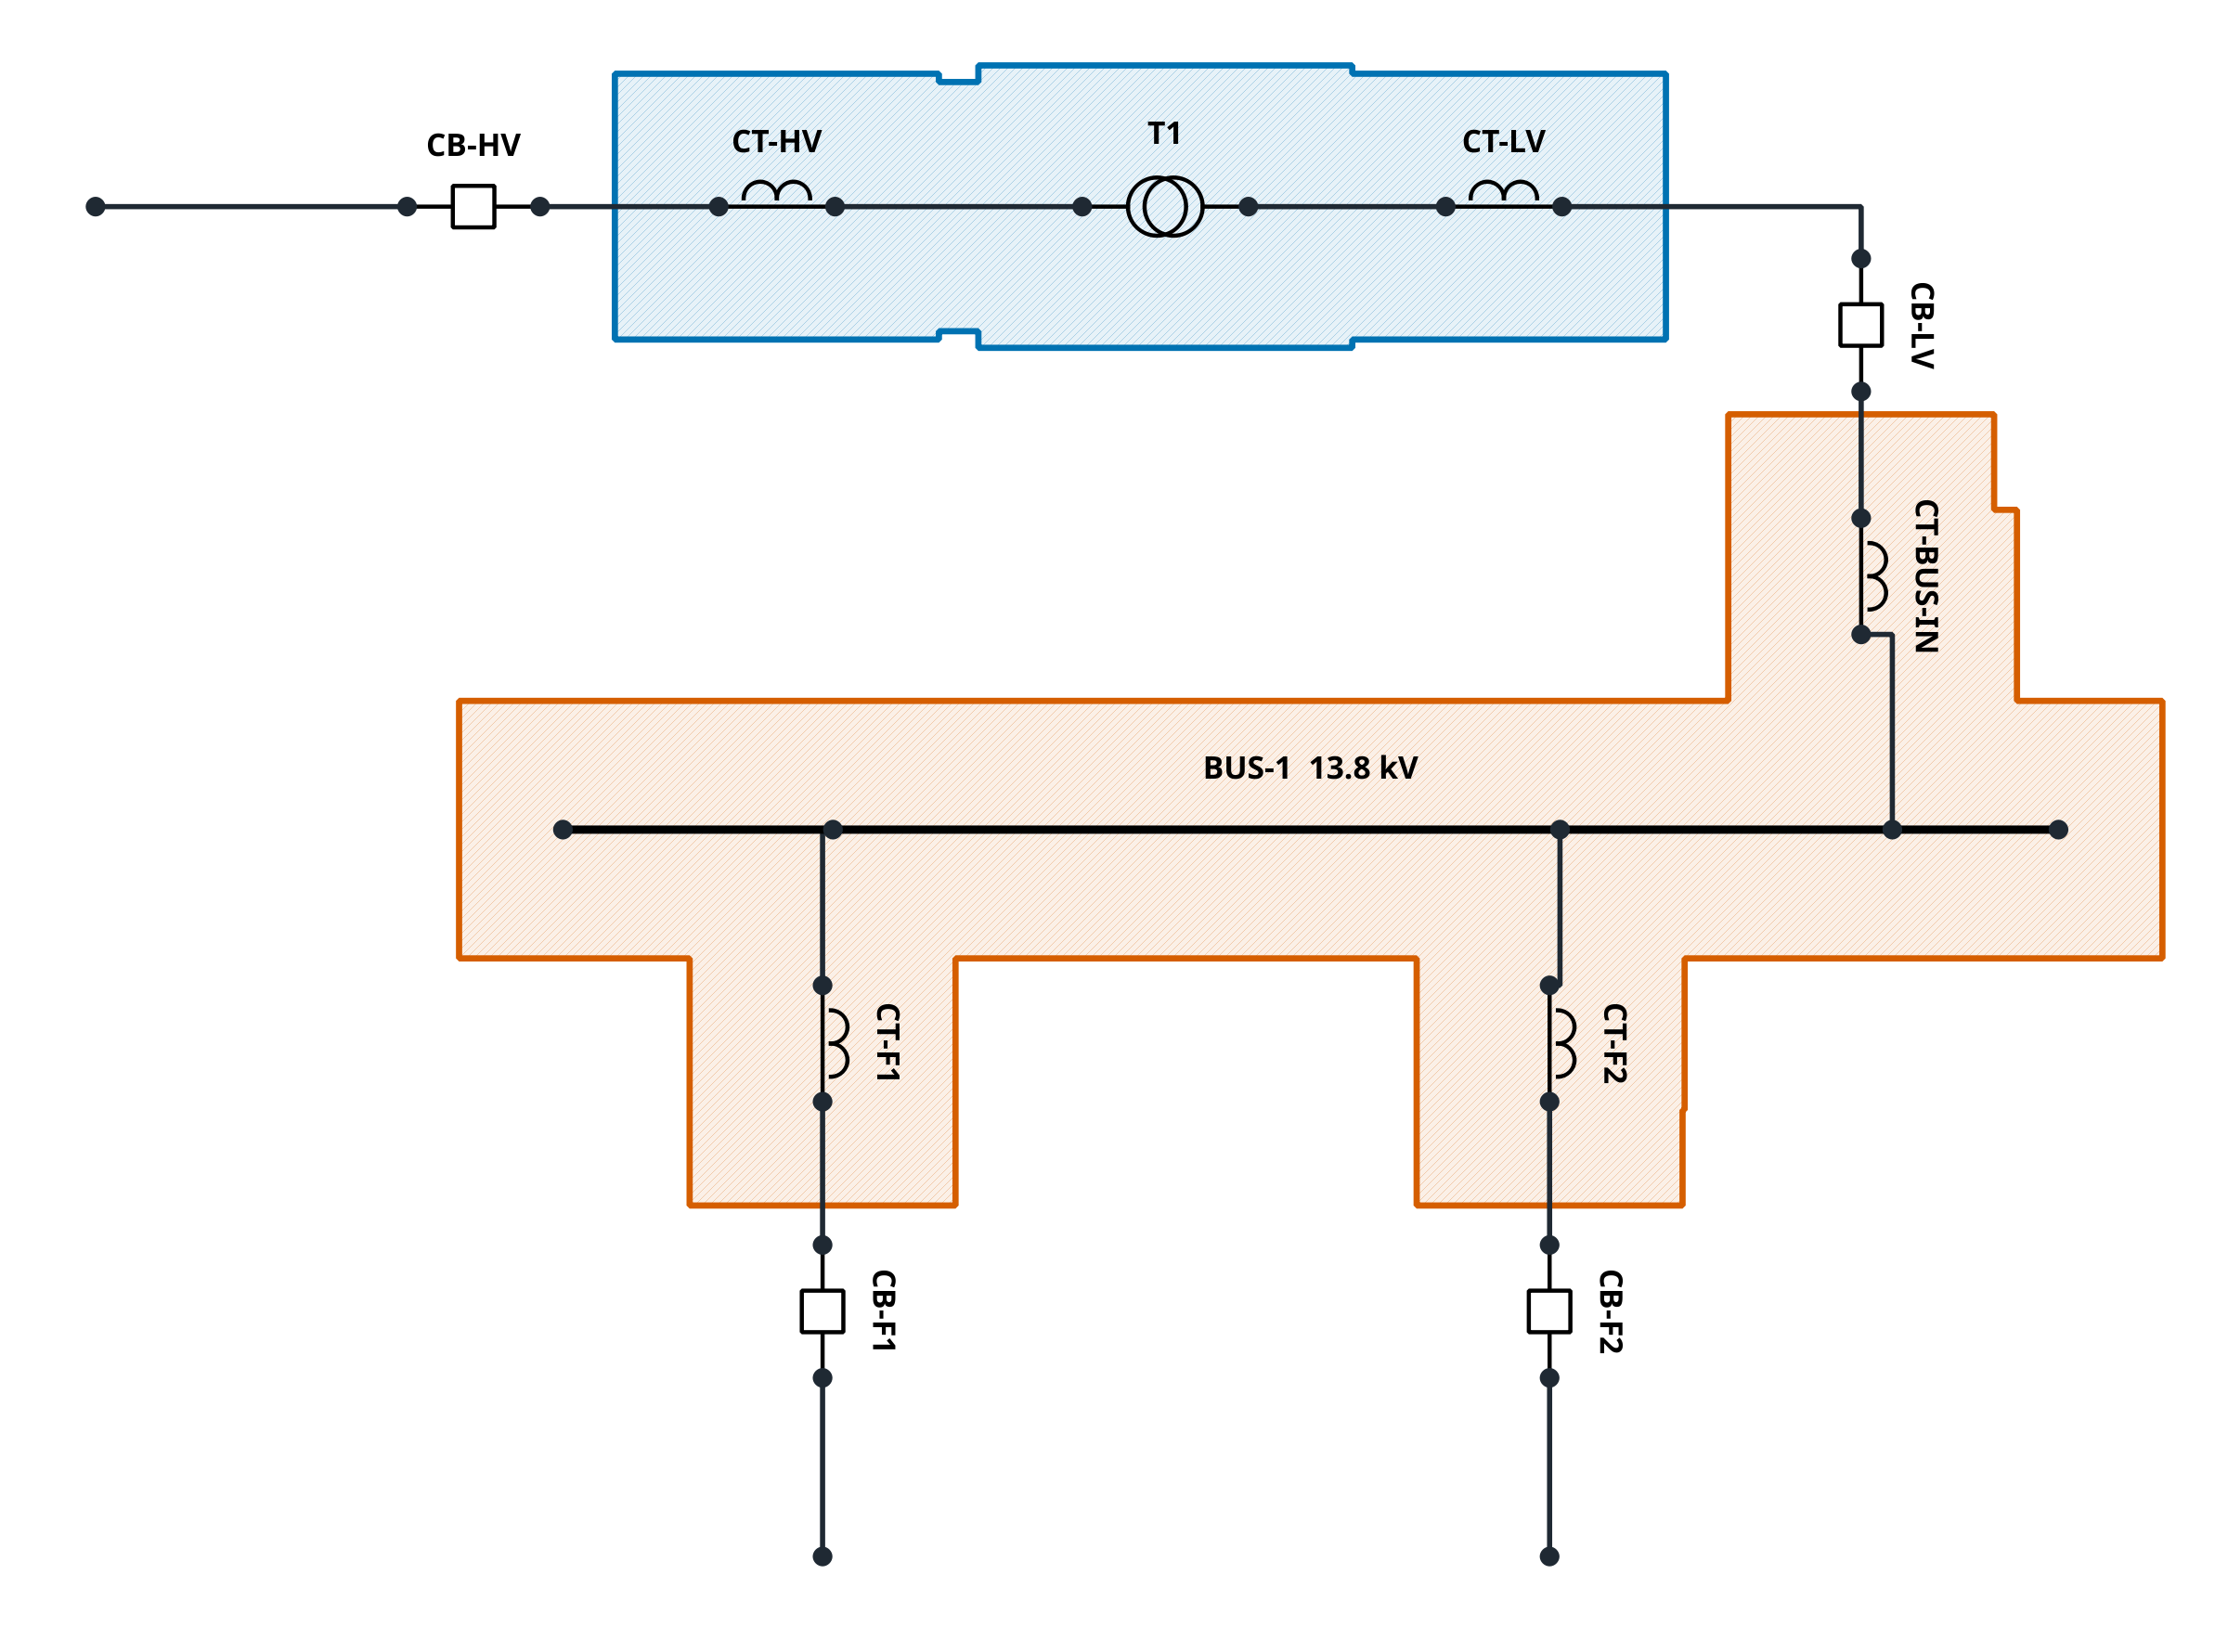
\includegraphics[width=0.8\textwidth]{images/demo_zones.png}
  \caption{Two-zone demonstration: transformer zone (blue) and bus zone (orange)}
  \label{fig:demo}
\end{figure}

\begin{table}[H]
  \centering
  \caption{Breaker currents in the demonstration (A)}
  \label{tab:democurrents}
  \begin{tabular}{l c c c c c}
    \toprule
    \textbf{Breaker} & \textbf{Trip Coil 1} & \textbf{Trip Coil 2} & \textbf{Close Coil} & \textbf{Motor Inrush} & \textbf{Motor Run} \\
    & (DC 1) & (DC 2) & (DC 1) & (DC 1) & (DC 1) \\
    \midrule
    CB-HV & 10 & 8 & --- & --- & --- \\
    CB-LV & 12 & 9 & --- & 18 & 3 \\
    CB-F1 & 6 & 5 & 10 & --- & --- \\
    CB-F2 & 7 & 6 & --- & --- & --- \\
    \bottomrule
  \end{tabular}
\end{table}

\paragraph{Transformer zone.} A transformer fault trips CB-HV and CB-LV, with both
coils operating together in the Primary trip stage:
\begin{align*}
  T_{\text{T1, trip, DC 1}} &= 10 + 12 = \SI{22}{A}, &
  T_{\text{T1, trip, DC 2}} &= 8 + 9 = \SI{17}{A}.
\end{align*}

\paragraph{Bus zone.} A bus fault trips CB-LV, CB-F1 and CB-F2. CB-F1 then recloses,
and CB-LV's spring-charging motor starts and runs:
\begin{align*}
  T_{\text{BUS, trip, DC 1}} &= 12 + 6 + 7 = \SI{25}{A}, &
  T_{\text{BUS, trip, DC 2}} &= 9 + 5 + 6 = \SI{20}{A},\\
  T_{\text{BUS, reclose, DC 1}} &= \SI{10}{A}, &
  T_{\text{BUS, inrush, DC 1}} &= \SI{18}{A}, \quad
  T_{\text{BUS, run, DC 1}} = \SI{3}{A}.
\end{align*}

\paragraph{Peaks.} Both zones are verified, so the study is complete, and
Equation~\ref{eq:peak} gives:
\begin{align*}
  P_{\text{DC 1}} &= \max(22,\,25,\,10,\,18,\,3) = \SI{25}{A} \quad\text{(bus zone, primary trip)},\\
  P_{\text{DC 2}} &= \max(17,\,20) = \SI{20}{A} \quad\text{(bus zone, primary trip)}.
\end{align*}

These match the tool's report exactly (Figure~\ref{fig:calcpdf}), as
Table~\ref{tab:demoresults} shows.

\begin{table}[H]
  \centering
  \caption{Demonstration results: hand calculation and tool}
  \label{tab:demoresults}
  \begin{tabular}{l l r r r r}
    \toprule
    \textbf{Zone} & \textbf{Stage} & \textbf{DC 1 (A)} & \textbf{DC 2 (A)} & \textbf{Total (A)} & \textbf{Tool} \\
    \midrule
    T1 Transformer Differential & Primary trip & 22 & 17 & 39 & 39 \\
    BUS-1 Bus Differential & Primary trip & 25 & 20 & 45 & 45 \\
    & Reclose & 10 & --- & 10 & 10 \\
    & Motor inrush & 18 & --- & 18 & 18 \\
    & Motor run & 3 & --- & 3 & 3 \\
    \midrule
    \multicolumn{2}{l}{\textbf{Supply peak}} & \textbf{25} & \textbf{20} & & \\
    \bottomrule
  \end{tabular}
\end{table}

The example illustrates three points that apply to every study:
\begin{itemize}
  \item CB-LV operates in both zones, but the zones are separate events, so its
        current is not added across them.
  \item The stage totals of \SI{39}{A} and \SI{45}{A} are not supply peaks, because
        they combine two supplies. Each battery sees only its own share.
  \item The reclose and motor currents are smaller than the trip currents here. Because
        they are separate stages, though, a large close coil or motor could set a
        supply's peak on its own.
\end{itemize}

\subsection{Assumptions and Limitations}

\begin{itemize}
  \item \textbf{Currents are entered, not derived.} The tool adds up the currents it
        is given. Reports state a nominal \SI{125}{V} DC system, but the voltage does
        not scale the currents, so enter currents for the DC voltage you intend.
  \item \textbf{Momentary current only.} The tool does not model duration, battery
        discharge or capacity in ampere-hours.
  \item \textbf{The engineer defines the sequence.} A stage occurs only if loads are
        assigned to it; the tool does not infer reclosing, breaker-failure or backup
        schemes. If loads in two stages can overlap in time, put them in the same stage.
  \item \textbf{Zones are proposals.} Detected zones follow the drawing's topology. The
        engineer must confirm the relay assignments and trip logic, which is why zones
        must be verified before results are final.
\end{itemize}
